
\documentclass{beamer}

\usepackage{algpseudocode, color, colortbl, listings, MnSymbol}

\usepackage{hyperref}
\hypersetup{
    colorlinks=true,
    urlcolor=blue,
}

\usetheme{Montpellier}
\usecolortheme{rose}

% page numbers, from
% https://tex.stackexchange.com/questions/137022/how-to-insert-page-number-in-beamer-navigation-symbols
\expandafter\def\expandafter\insertshorttitle\expandafter{%
  \insertshorttitle\hfill%
  \insertframenumber\,/\,\inserttotalframenumber}

\definecolor{Gray}{gray}{0.8}
\newcolumntype{g}{>{\columncolor{Gray}}c}

\newcommand{\stanza}{ \\~\ }

\title{17. Approximation and Vertex Cover}
\subtitle{CPSC 535}
\author{Kevin A. Wortman}
\institute{ 
\includegraphics[height=2cm]{csuf-logo-cmyk} }
\date{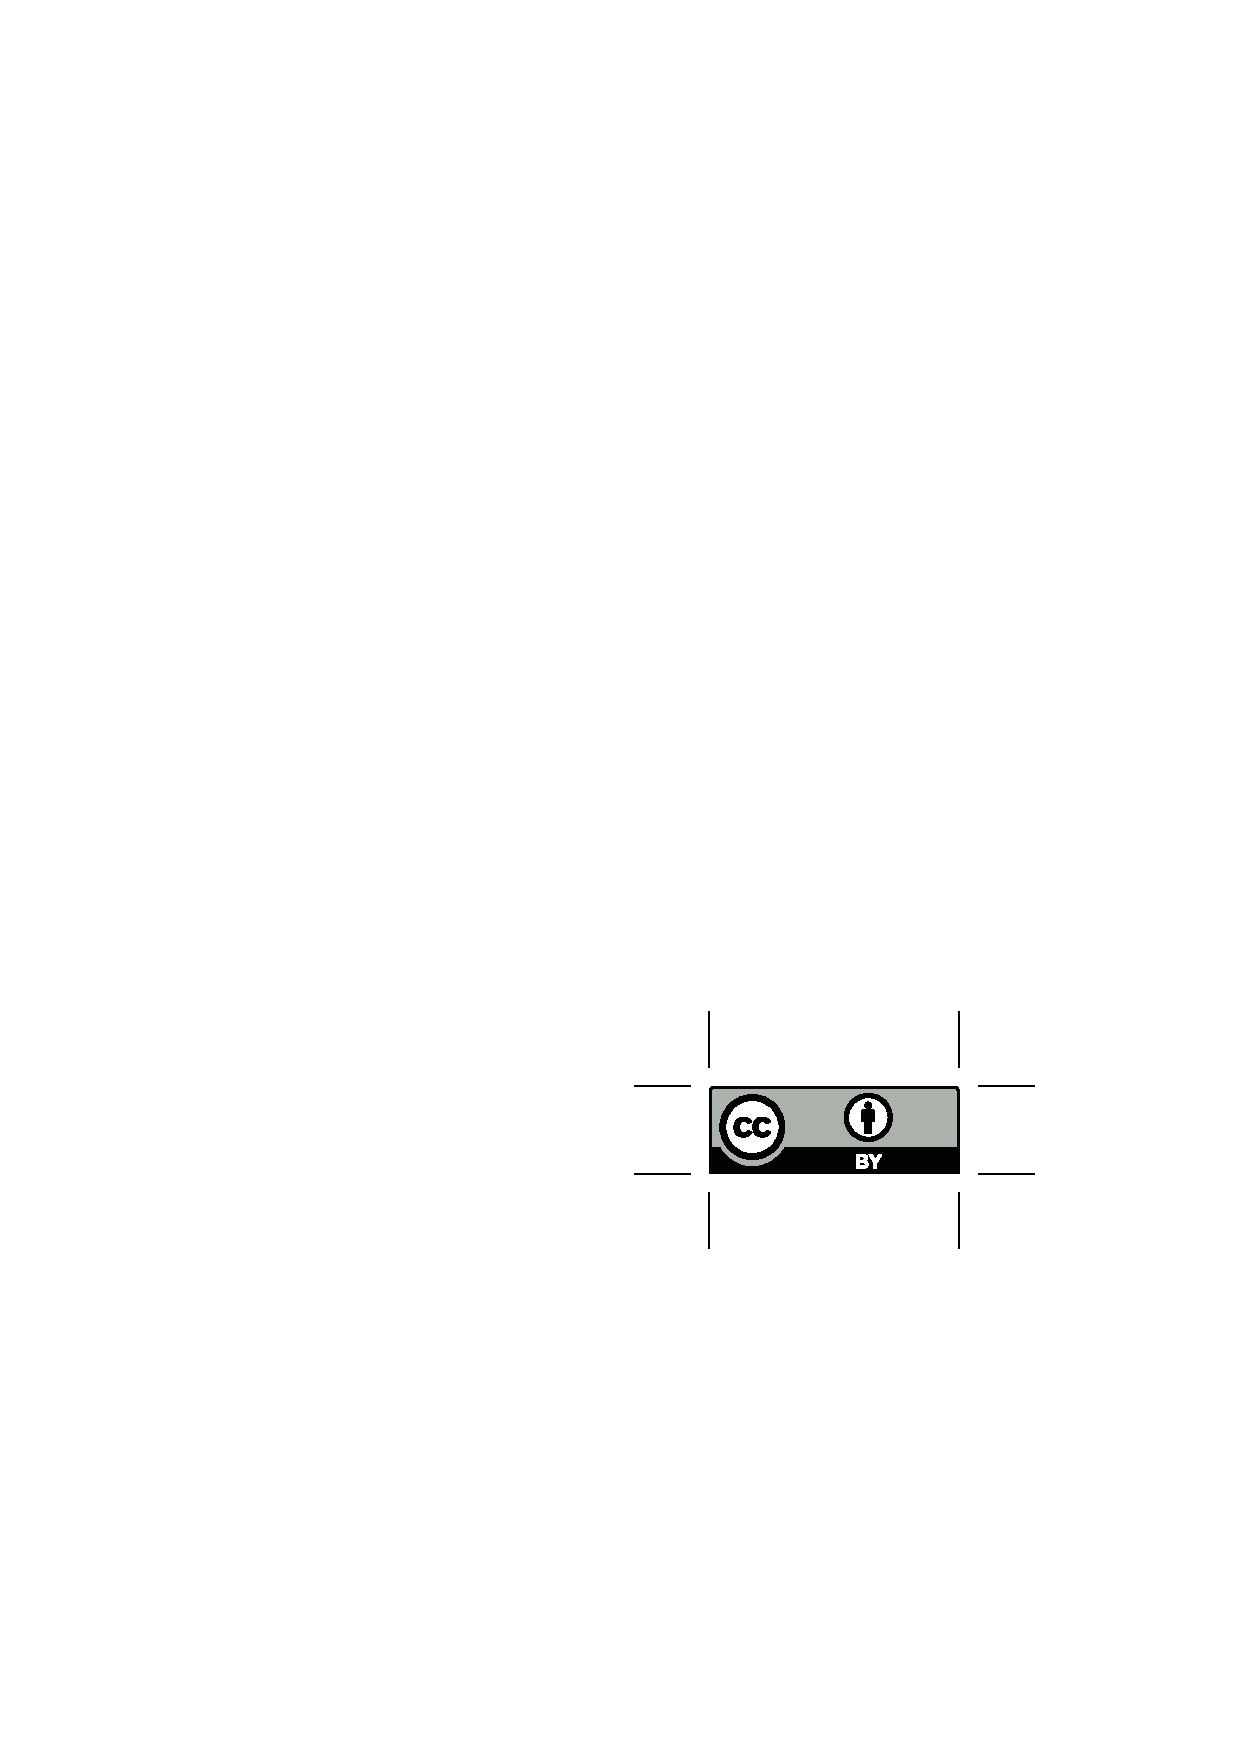
\includegraphics[height=14pt]{by} \\

{\tiny
This work is licensed under a
\href{http://creativecommons.org/licenses/by/4.0/}{Creative Commons Attribution 4.0 International License}.
}}

\begin{document}

\begin{frame}
  \titlepage
\end{frame}

\begin{frame} \frametitle{Big Idea: Renegotiating Problems}
Sometimes we want to solve a problem, but there is an obstacle
\begin{itemize}
  \item computational complexity: problem is $NP$-hard or undecidable
  \item ill-posed: don't know how to phrase problem as precise input/output statement
\end{itemize}

These are insurmountable; progress not possible. \stanza

Sometimes we can \emph{negotiate} on the definition of the problem
\begin{itemize}
  \item adjust input/output def'n to correspond to an easier problem
  \item more specific input; or more general output
  \item ideally, computational problem still helps with the business problem
  \item combines CS hard skills with business soft skills
\end{itemize}
\end{frame}

\begin{frame} \frametitle{Approximation}
\textbf{Approximation}: output is \emph{nearly-optimal} but not necessarily
truly optimal.
\begin{itemize}
  \item quality is quantified, \textbf{proven}
  \item ``approximation'', ``approximate'' are technical terms; use other words
    like ``decent'' for informal ideas about quality
  \item suitable for use cases where approximate solutions are adequate
  \item need to rewrite problem definition
  \item every optimization problem has corresponding approximation problems; but these
    are distinct problems
\end{itemize}
\end{frame}

\begin{frame} \frametitle{Example: optimal vs. approximate graph coloring}
\emph{graph coloring} \\
\textbf{input}: connected graph $G=(V,E)$ \\
\textbf{output}: coloring $c$ using $k$ colors, where each vertex $v \in V$ is assigned color
  $c(v) \in \{1, \ldots k\},$ no pair of adjacent vertices are assigned the
  same color, and the number of colors $k$ is minimal
\stanza

\emph{3-approximate graph coloring} \\
\textbf{input}: connected graph $G=(V,E)$ \\
\textbf{output}: coloring $c$ using $k$ colors, where each vertex $v \in V$ is assigned color
  $c(v) \in \{1, \ldots k\},$ no pair of adjacent vertices are assigned the
  same color, \textbf{and the number of colors $k$ satisfied $k \leq 3 k^\star$,
  where $k^\star$ is the fewest colors possible for $G$}
\end{frame}

\begin{frame} \frametitle{Graph Coloring Example}
  \begin{center}
    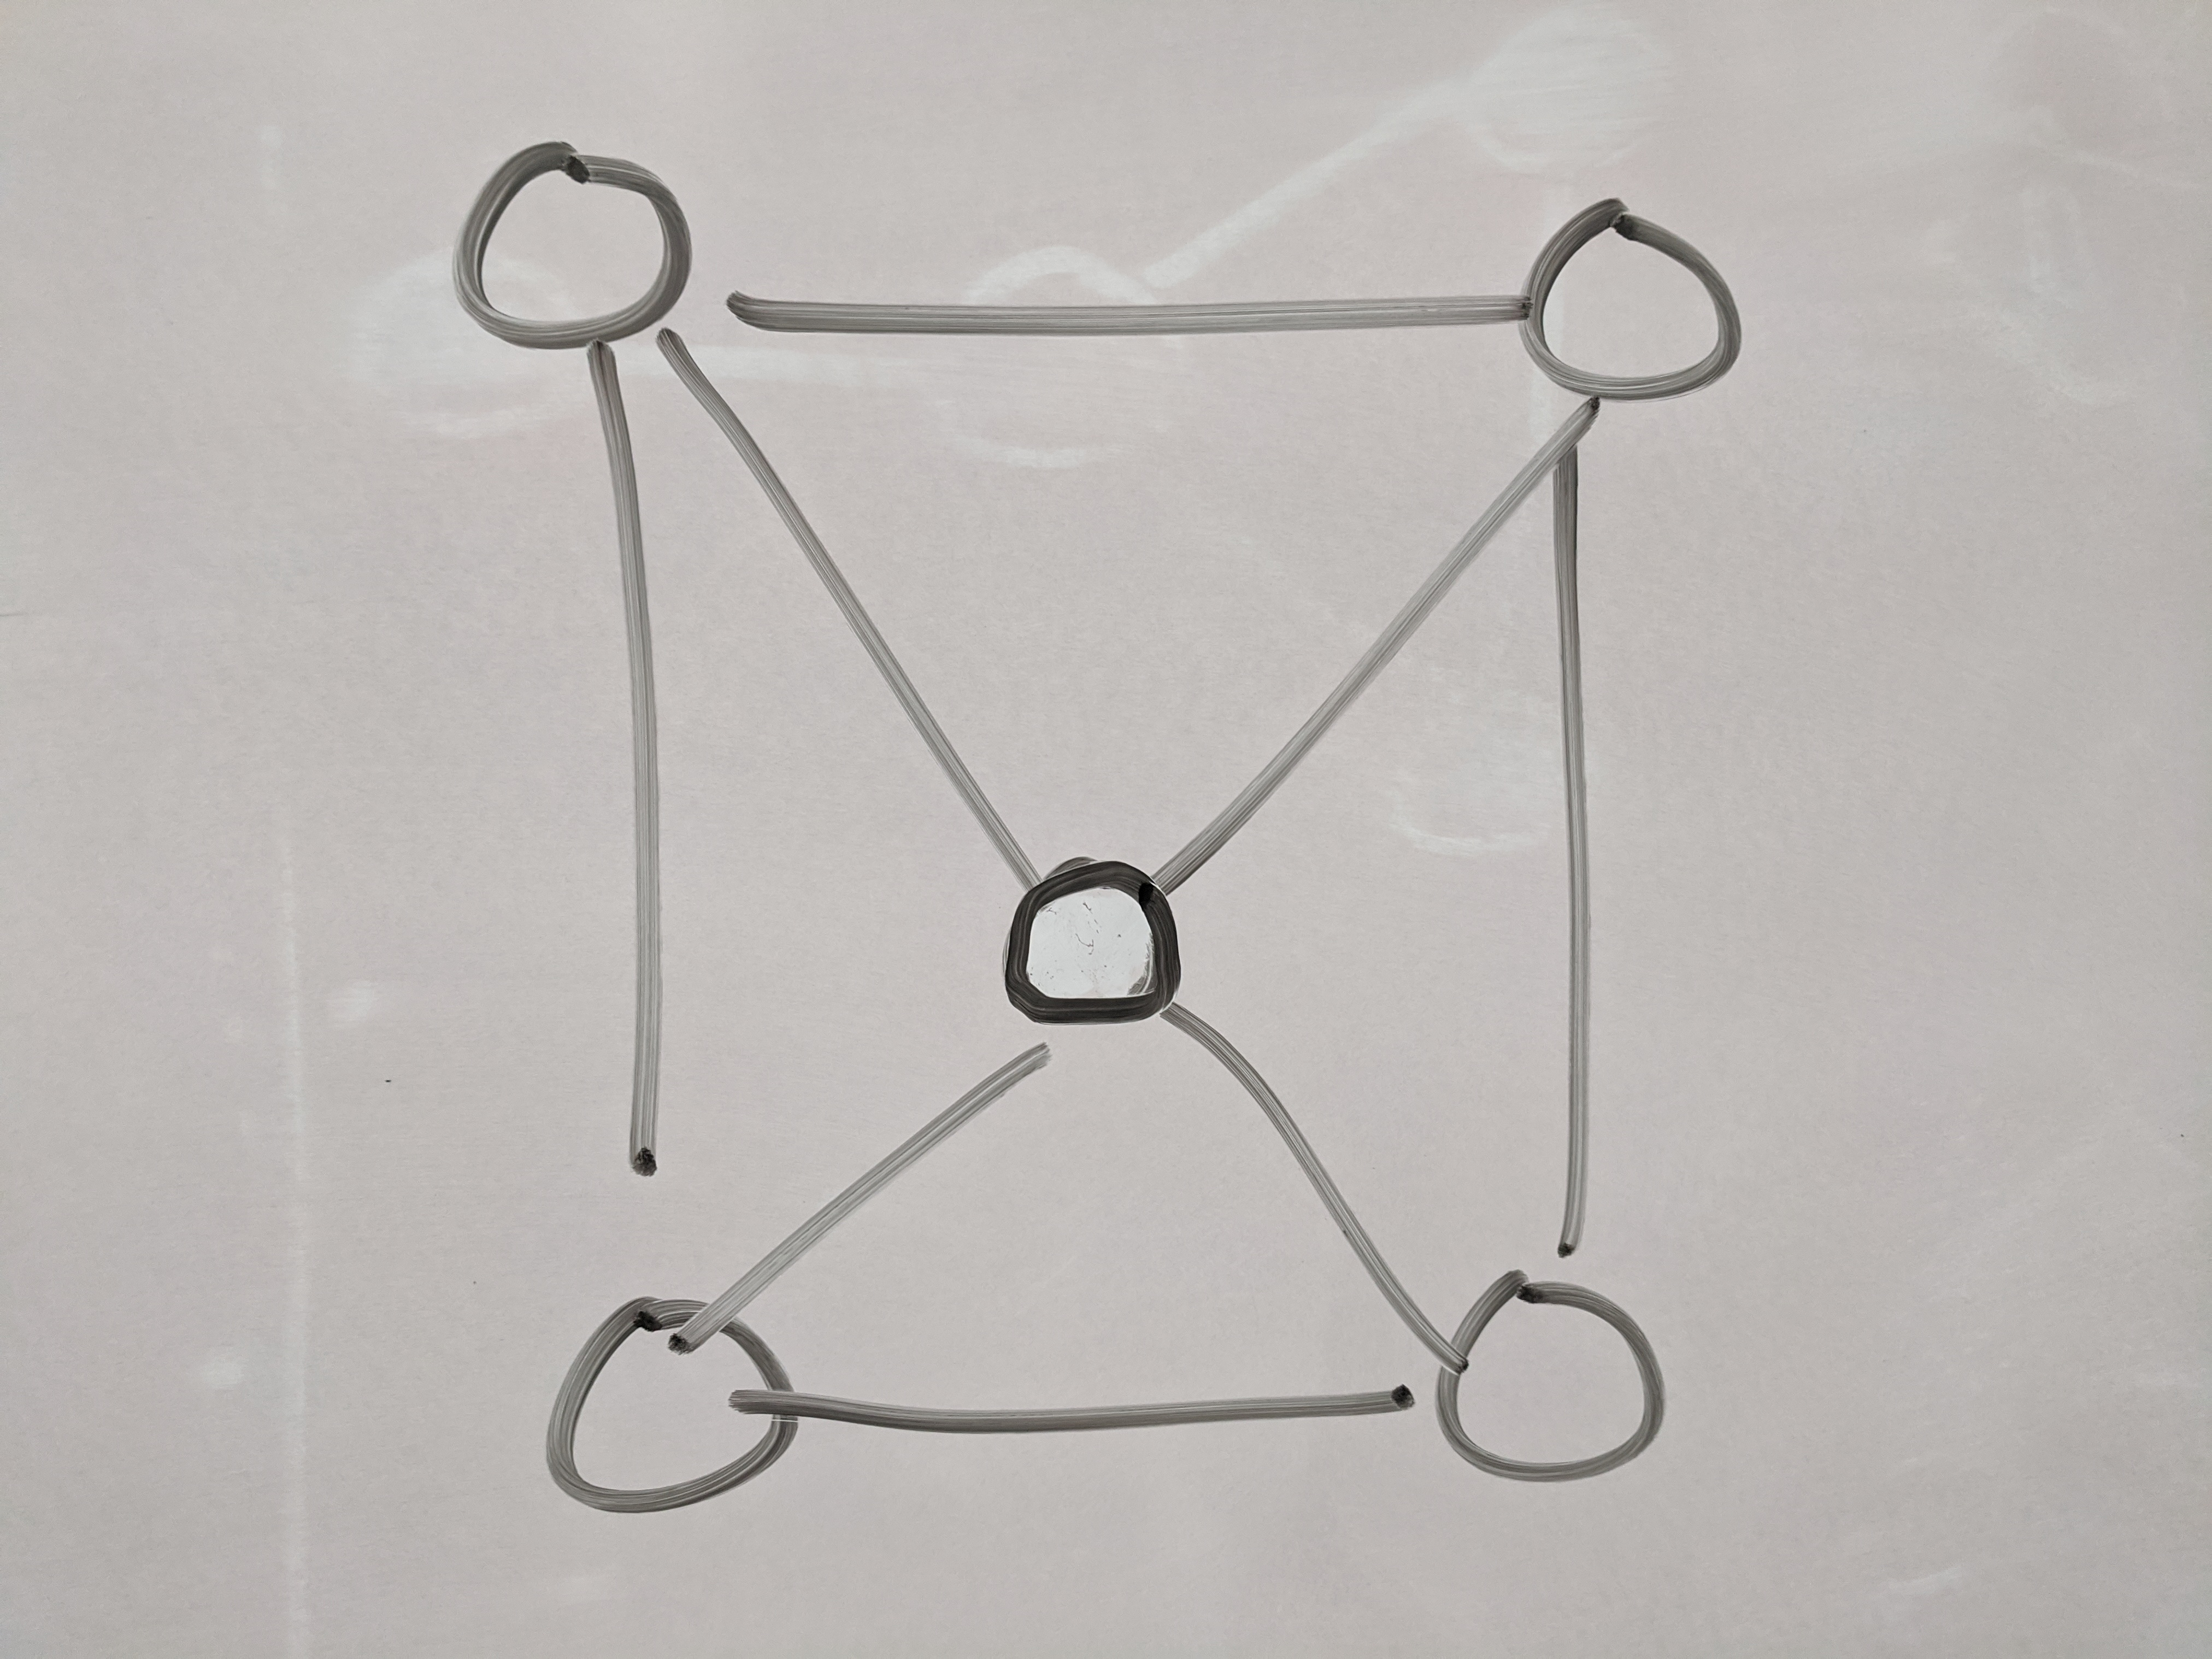
\includegraphics[height=100pt]{13-graph-uncolored.jpg}
    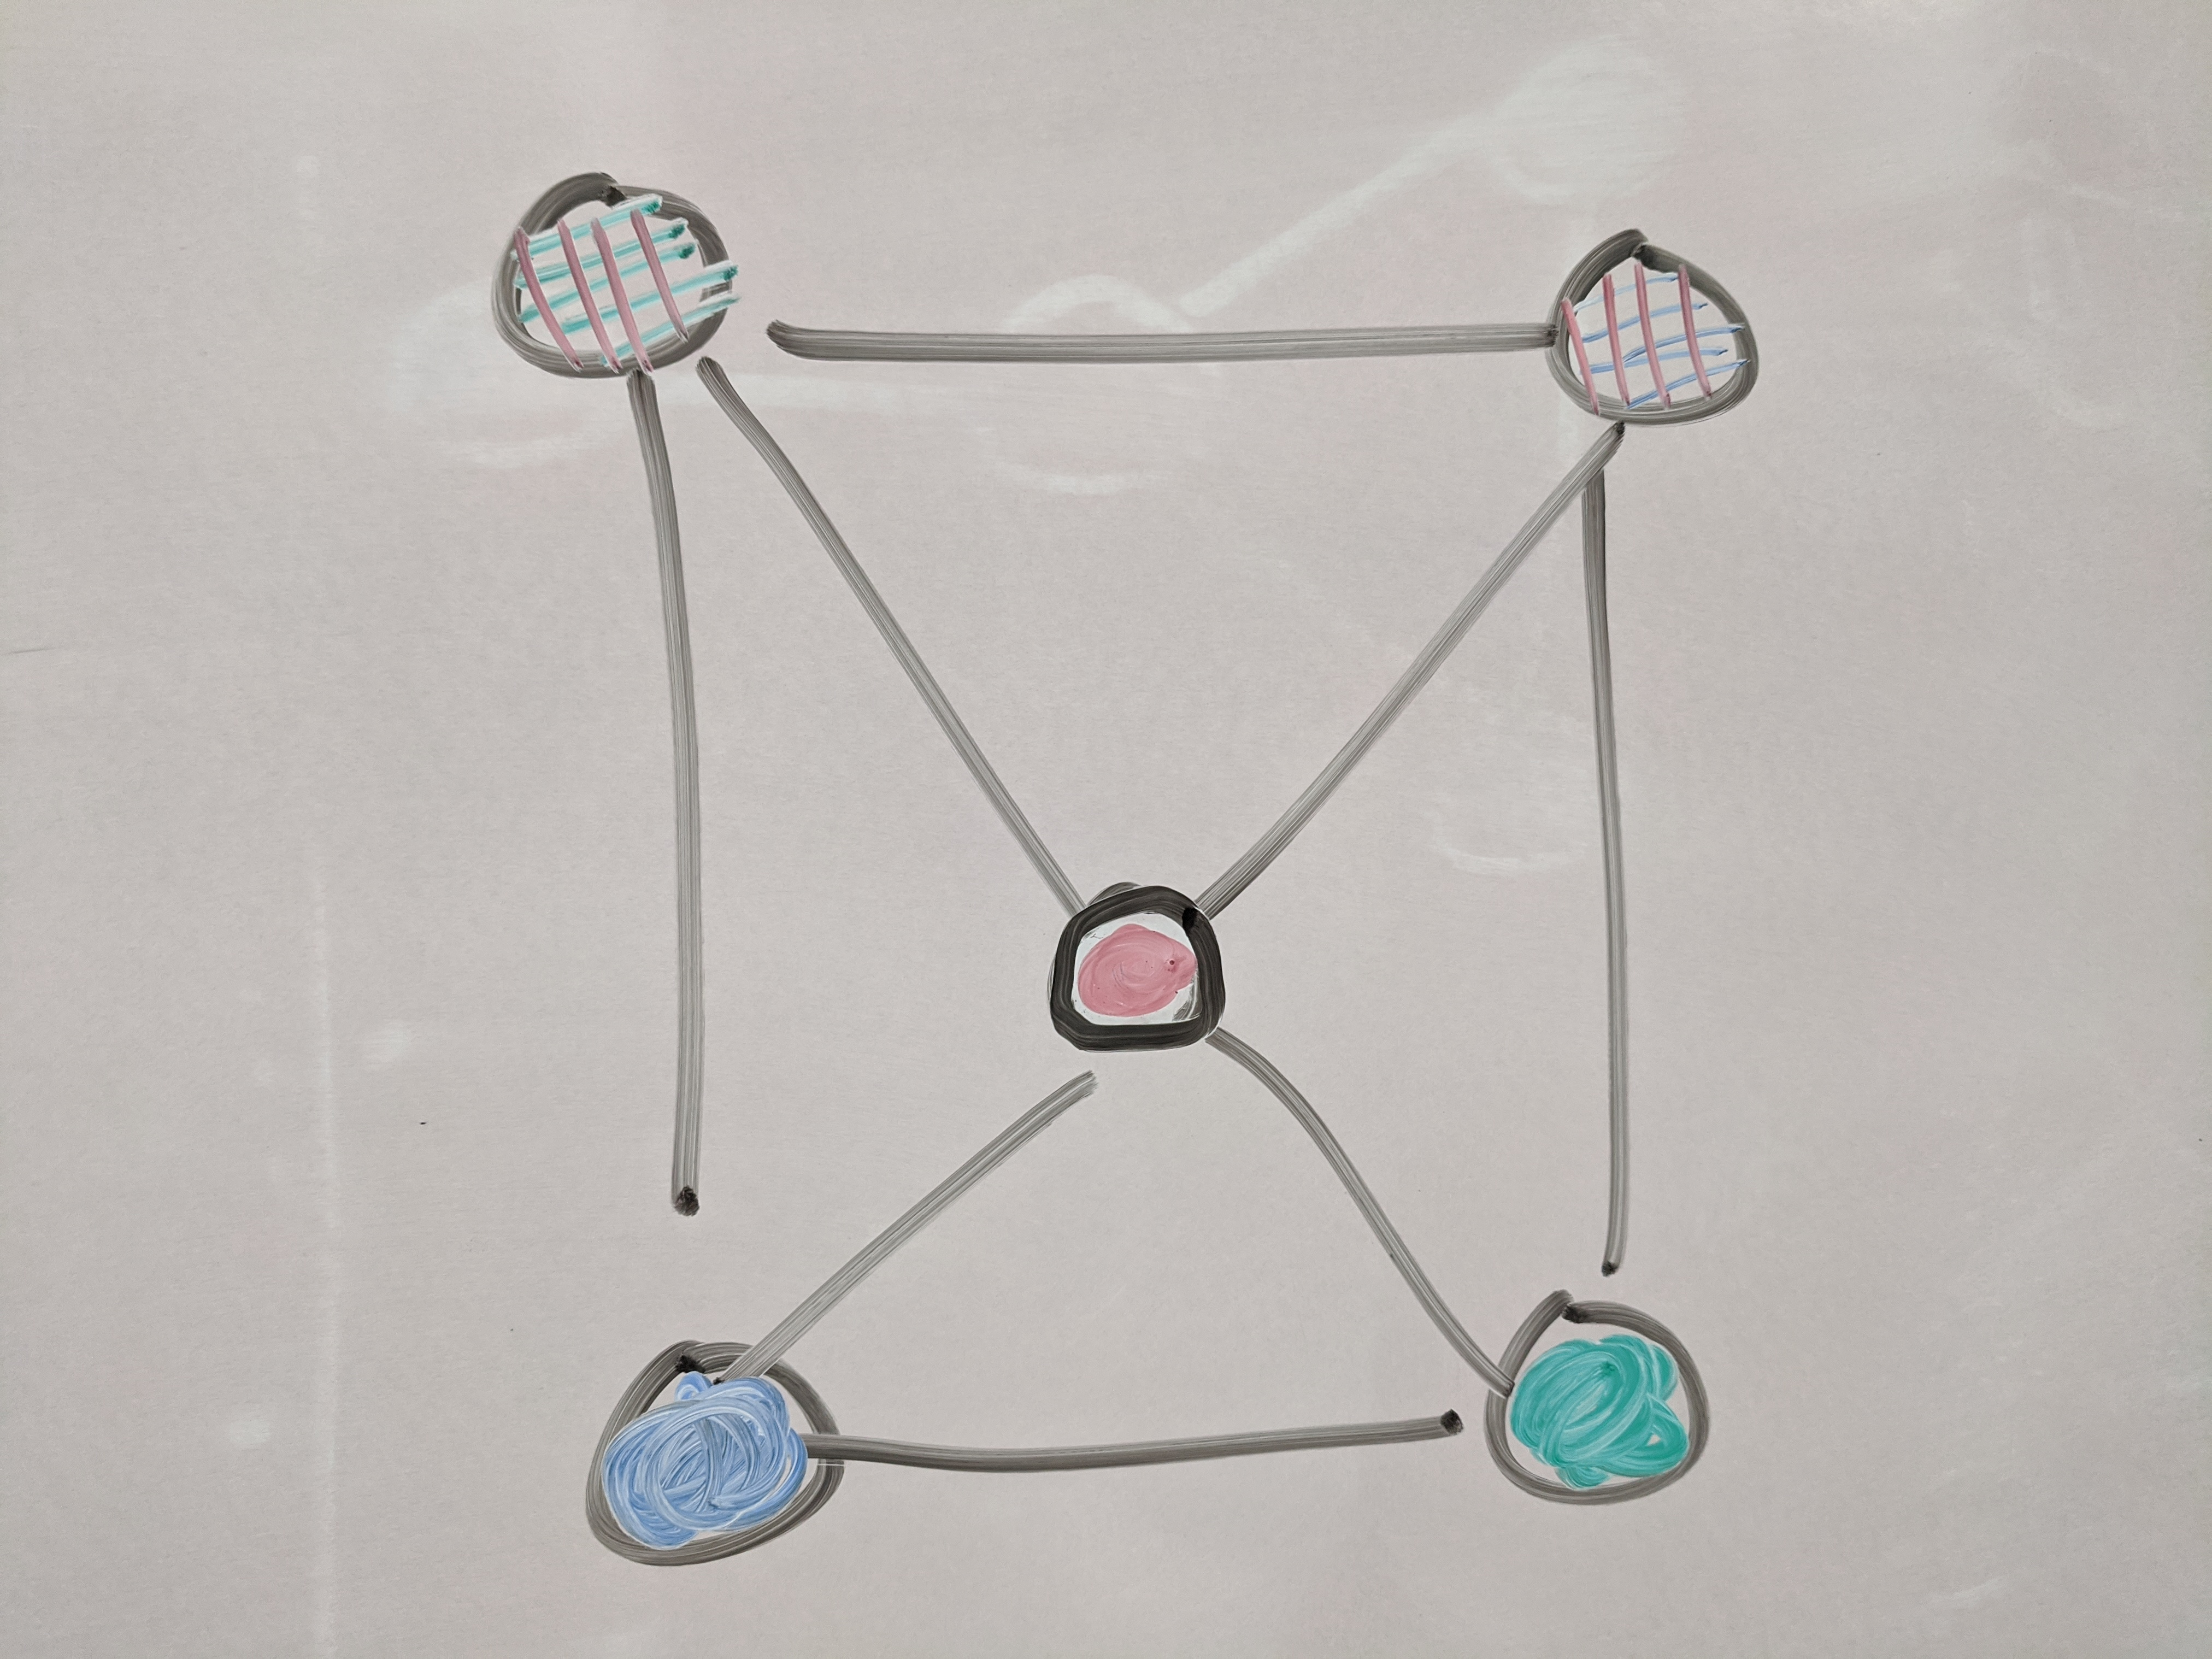
\includegraphics[height=100pt]{13-graph-colored-suboptimal.jpg}
    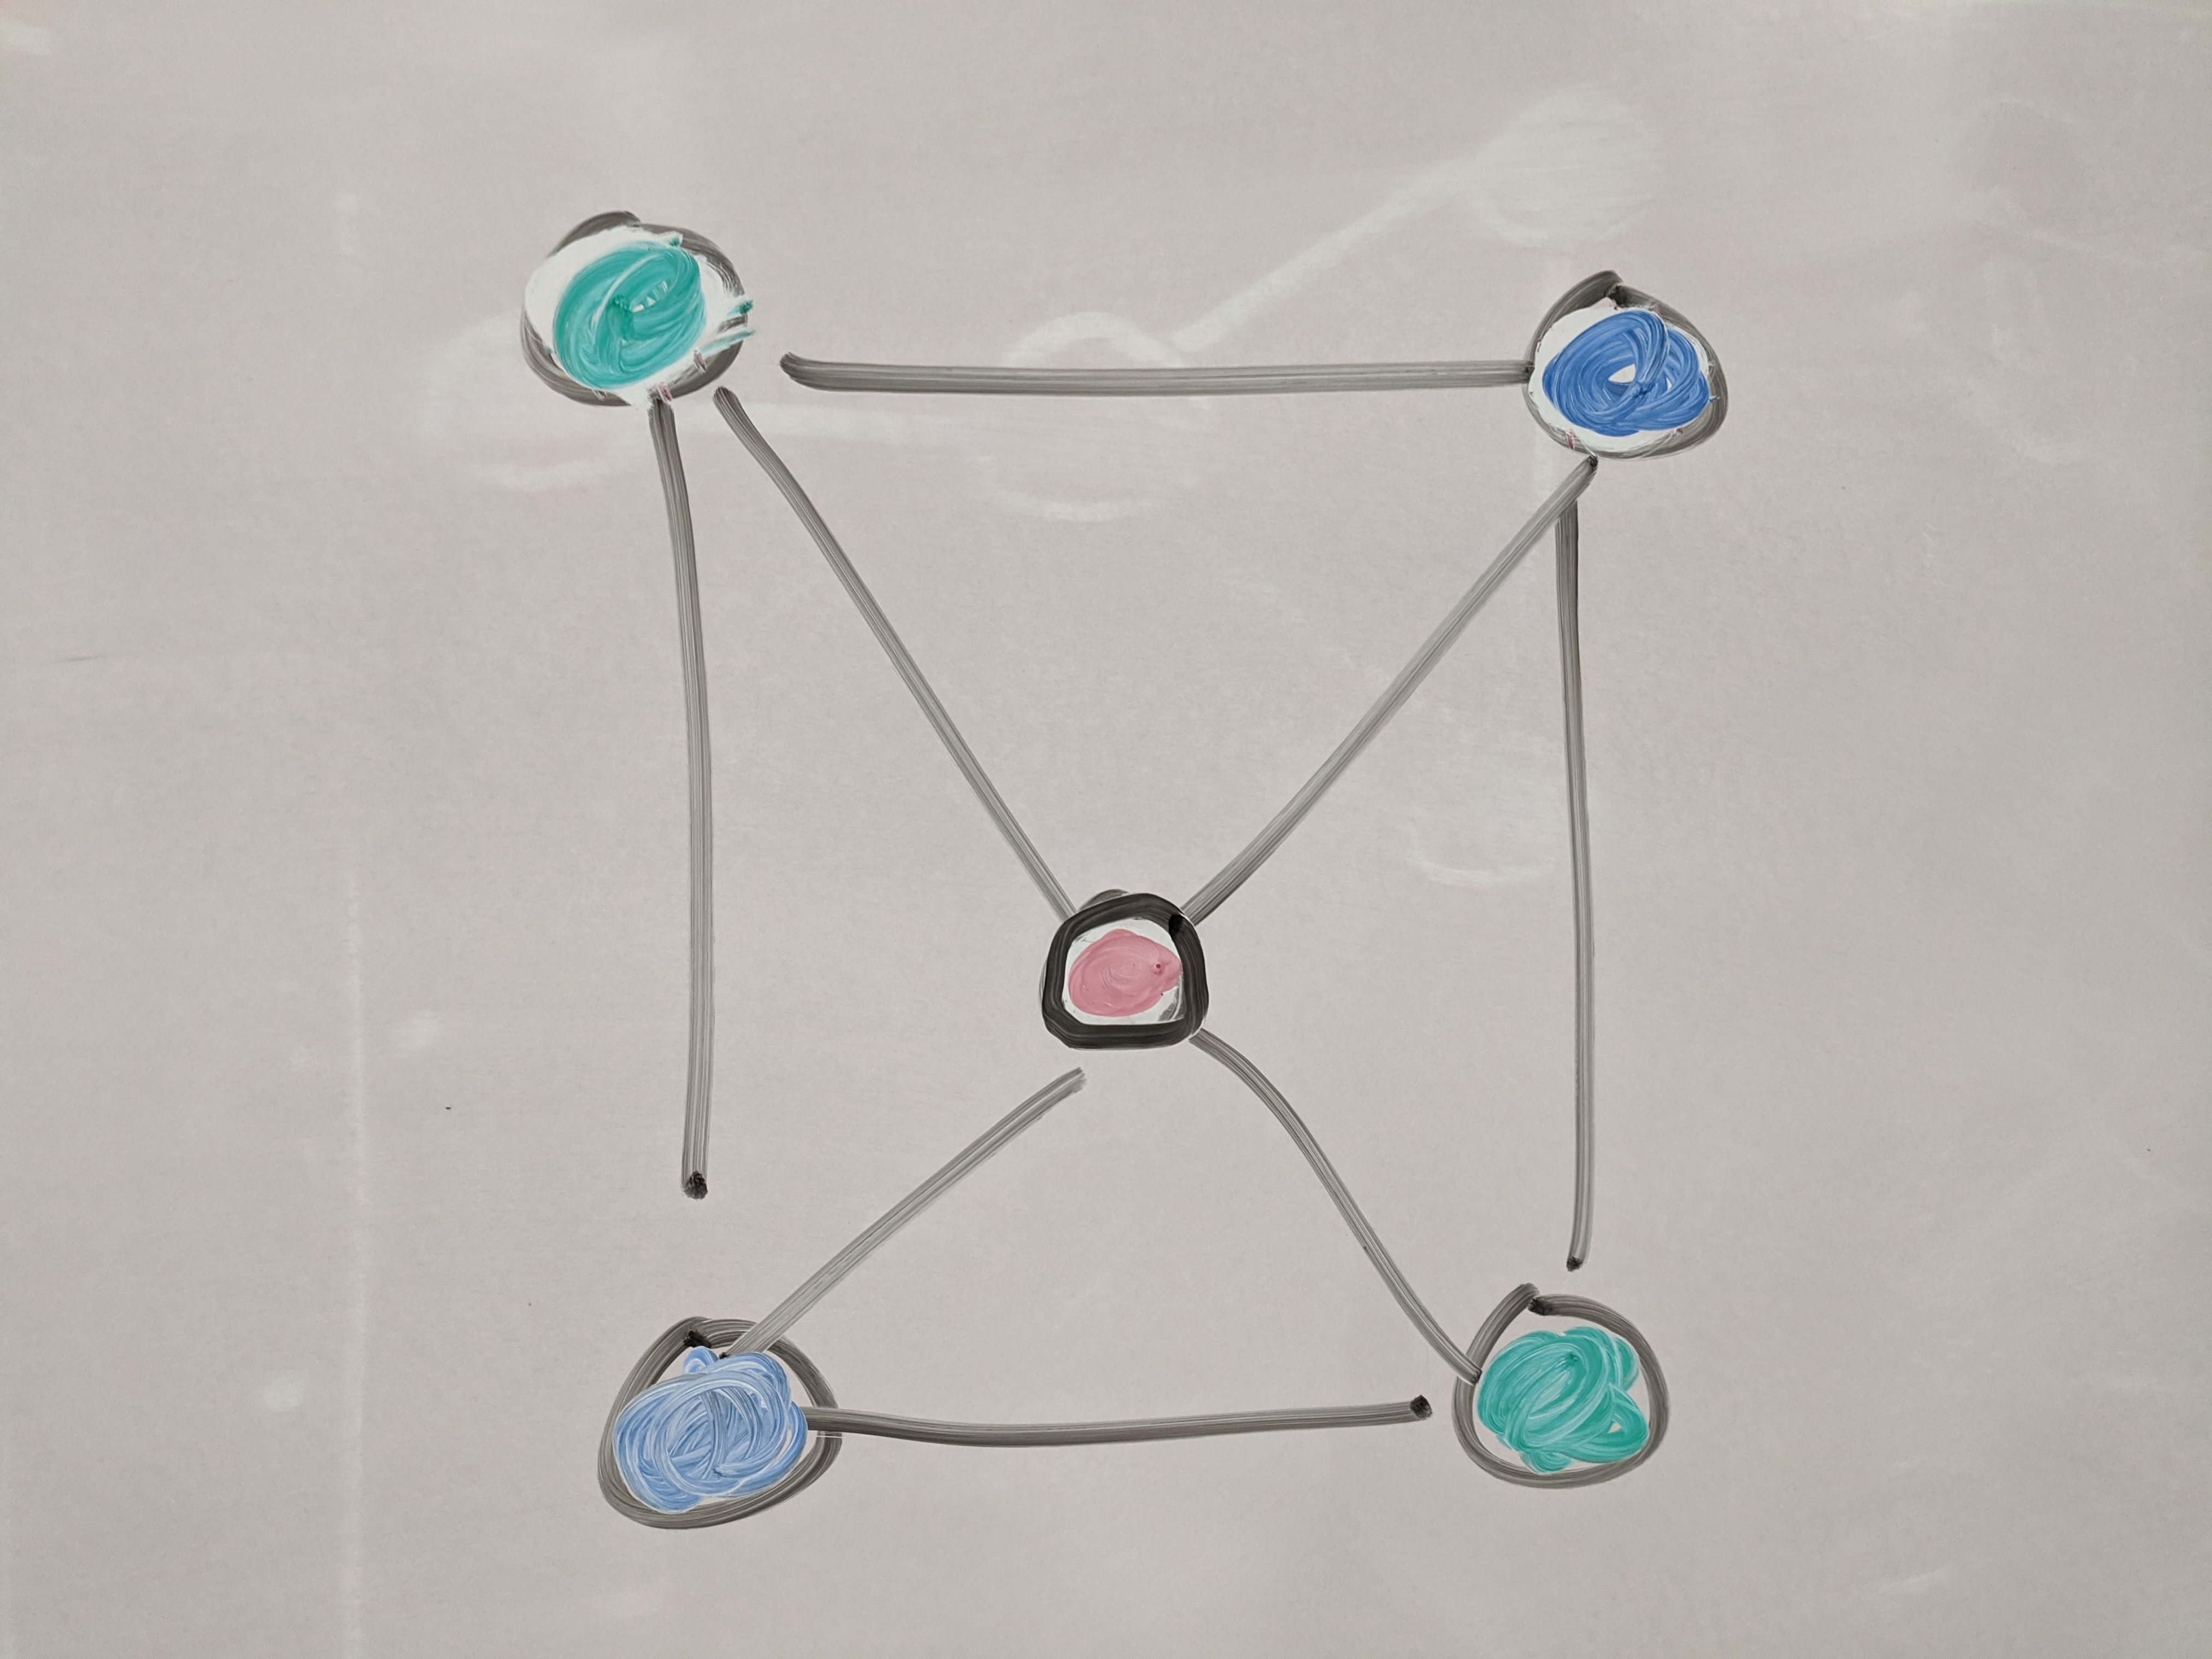
\includegraphics[height=100pt]{13-graph-colored-optimal.jpg}
  \end{center}
\end{frame}

\begin{frame} \frametitle{Approximation vs. Other Renegotiation Approaches}
Other ways of dealing with hard problems:
\begin{itemize}
  \item say ``no''
  \item when $n$ is small enough, just use exponential-time algorithm
  \item no \emph{proof} of solution quality, but nonetheless sometimes good enough:
    \begin{itemize}
      \item machine learning algorithms (also, in M.L. humans don't need to precisely define what counts as ``correct'')
      \item fast heuristic algorithms
      \item Monte Carlo algorithms
    \end{itemize}
\end{itemize}

Approximation
\begin{itemize}
  \item pros: \emph{provable} solution quality, often fast
  \item con: human needs to design and analyze algorithm for each specific problem
\end{itemize}
\end{frame}

\begin{frame} \frametitle{Performance Ratios}
\textbf{Approximation ratio} $\rho(n)$: ratio between quality of algorithm's output
and optimal output; smaller is better
\begin{itemize}
  \item for \textbf{maximization} problem: if optimal quality is $C^\star$ and alg. produces
    quality $C,$ by definition $C^\star \geq C,$ and define
    \[ \rho(n) = \frac{C^\star}{C} \]
  \item for \textbf{minimization} problem: if optimal quality is $C^\star$ and alg. produces
    quality $C,$ by definition $C^\star \leq C$ and define
    \[ \rho(n) = \frac{C}{C^\star} \]
\end{itemize}
Recall 3-approx. vertex cover: output \# colors $\leq 3 k^\star$
\end{frame}

\begin{frame} \frametitle{Fixed Approximation Ratios}
Some approxmation algorithms have a fixed approximation ratio that is
``baked in'' to the design of the algorithm. \stanza

Ex.: algorithm that solves 3-approx. vertex cover would have fixed $\rho(n)=3$
\stanza

In general, better (smaller) ratios require slower algorithms. \\
(note 1-approximation algorithms produce optimal solutions.) \stanza

Deriving a different quality-vs.-time trade-off requires designing an
entirely different algorithm.
\end{frame}

\begin{frame} \frametitle{Approximation Schemes}
\textbf{approximation scheme}: family of related algorithms, such that, for
any parameter $\epsilon > 0,$ scheme defines a
$(1+\epsilon)$-approximate algorithm
\begin{itemize}
  \item think of $\epsilon$ as being a \textbf{const} variable
  \item time-performance trade-off is fully tuneable at compile time
\end{itemize}

\textbf{Polynomial Time Approximation Scheme (PTAS)}: approx. scheme where runtime
is polynomial in $n$; nothing said of relationship to $\epsilon$ \\
e.g. $O(2^{1/\epsilon} n \log n)$ \stanza

\textbf{Fully PTAS}: runtime is polynomial in $n$ and $1/\epsilon$ \\
e.g. $O((1/\epsilon)^2 n^3)$
\end{frame}

\begin{frame} \frametitle{Vertex Cover Problem}
\emph{vertex cover problem} \\
\textbf{input}: undirected graph $G=(V,E)$ \\
\textbf{output}: set of vertices $C \subseteq V$, of minimal size $|C|,$ such
  that every edge in $E$ is incident on at least one vertex in $C$
 \stanza

 \emph{2-approximate vertex cover problem} \\
 \textbf{input}: undirected graph $G=(V,E)$ \\
 \textbf{output}: set of vertices $C \subseteq V$, such
   that every edge in $E$ is incident on at least one vertex in $C$, and
   $|C| \leq 2 |C^\star|$ where $C^\star$ is a minimal vertex cover for $G$
  \stanza

See Wiki page: \url{https://en.wikipedia.org/wiki/Vertex_cover}
\end{frame}

\begin{frame} \frametitle{Vertex Cover Example}
  \begin{center}
    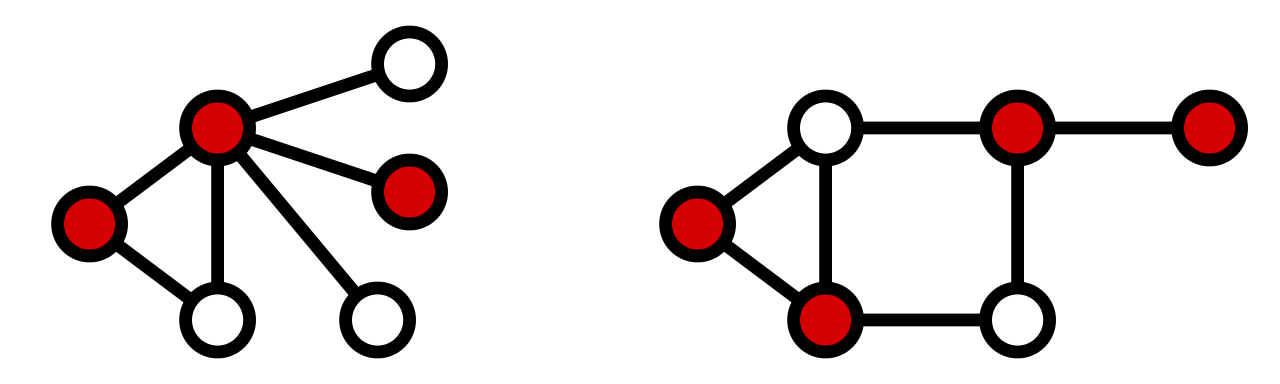
\includegraphics[height=80pt]{13-vertex-cover-1.png}
    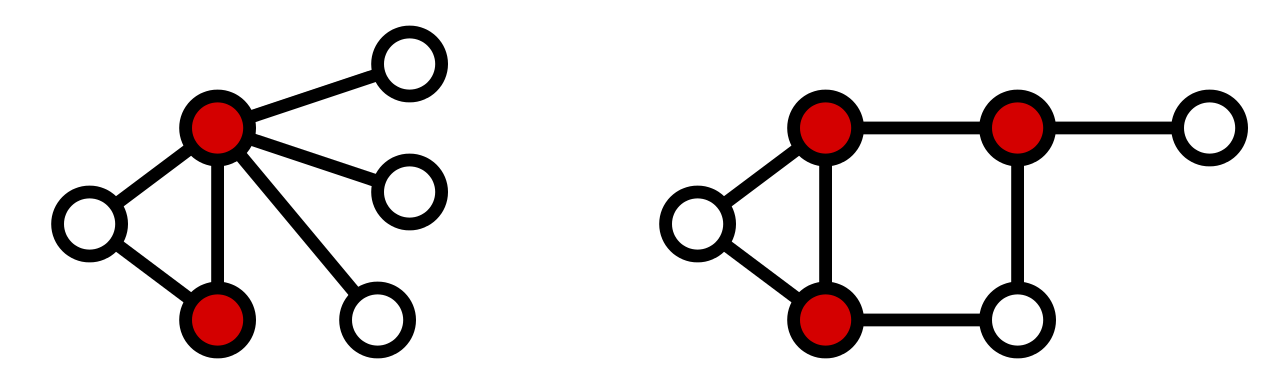
\includegraphics[height=80pt]{13-vertex-cover-2.png}
  \end{center}

  {\tiny
  Images credit: Wikipedia user Miym,
  \href{https://creativecommons.org/licenses/by-sa/3.0)}{CC BY-SA 3.0},
  \url{https://commons.wikimedia.org/wiki/File:Vertex-cover.svg},
  \url{https://commons.wikimedia.org/wiki/File:Minimum-vertex-cover.svg}
  }
\end{frame}

\begin{frame} \frametitle{Vertex Cover Hardness}
  \begin{itemize}
    \item vertex cover is $NP$-complete
    \item baseline algorithm:
    \begin{itemize}
      \item exhaustive search
      \item for each subset $C$ of vertices, check whether every edge has an
        endpoint in $C$
      \item return the smallest $C$ that is a valid cover
      \item $\Theta(2^n m)$ time, exponential, slow
    \end{itemize}
    \item goal of a 2-approximate vertex cover algorithm:
    \begin{itemize}
      \item get a decent (though imperfect) cover much faster
    \end{itemize}
  \end{itemize}
\end{frame}

\begin{frame} \frametitle{A Greedy Approximation Algorithm}
Idea:
\begin{itemize}
  \item every edge $e=(u,v)$ needs both $u \in C$ and $v \in C$
  \item so grab an edge $e=(u,v)$ and include $u$ and $v$ in $C$
  \item every other edge touching $u$ or $v$ is now covered, so eliminate them
  \item continue until every edge is either grabbed or eliminated
  \item good: definitely finds a correct cover $C$
  \item bad: depending on the order of the ``grabs'', heuristic can get tricked
    into picking sub-optimal vertices
\end{itemize}
\end{frame}

\begin{frame} \frametitle{2-Approximate Vertex Cover Pseudocode}
  \begin{algorithmic}[1]
    \Function{APPROX-VERTEX-COVER}{$G=(V,E)$}
      \State $C=\emptyset$
      \State $T=E$ \Comment{$T = $ edges that may be taken}
      \While { $T \ne \emptyset$ }
        \State Let $e=(u, v)$ be an arbitrary edge in $T$
        \State $C = C \cup \{u, v \}$
        \State Remove from $T$ any edge $f$ that is incident on $u$ or $v$
      \EndWhile
      \State \Return $C$
    \EndFunction
  \end{algorithmic}
\vspace{.5cm}
\textbf{Efficiency Analysis}: $O(m+n)$ time (assuming efficient data structures
for $G, T,$ and $C$)
\end{frame}

\begin{frame} \frametitle{Vertex Cover Performance Ratio}
\textbf{Lemma}: APPROX-VERTEX-COVER is a 2-approximation algorithm. \\
\textbf{Need:} for any $G, |C| \leq 2 |C^\star|$ \\
\textbf{Proof sketch}:
\begin{itemize}
  \item Let $A$ be the set of edges chosen inside the \textbf{while} loop
  \item will bound $|C|, |C^\star|$ both in terms of $|A|$
\end{itemize}
\end{frame}
  
\begin{frame} \frametitle{Vertex Cover Performance Ratio (cont'd)}
\begin{itemize}
  \item \textbf{(1)} $|C^\star|$ vs. $|A|$
  \item $C^\star$ is a vertex cover, so for every edge $(u, v) \in A,$ we must have
    $u \in C^\star$ and/or $v \in C^\star$
  \item the ``Remove from $T$'' step guarantees that, after $(u, v)$ is chosen,
    no other edge incident on $u$ or $v$ will be chosen and added to $A$
  \item $\Rightarrow$ each vertex $x \in C^\star$ covers \emph{exactly} one edge in $A$
  \item $\Rightarrow |C^\star| \geq |A|$
\end{itemize}
\end{frame}

\begin{frame} \frametitle{Vertex Cover Performance Ratio (cont'd)}
\begin{itemize}
  \item \textbf{(2)} $|C|$ vs. $|A|$
  \item the $C = C \cup \{u, v \}$ step inserts 2 vertices into $C$
  \item  due to the same ``Remove from $T$'' logic, neither $u$ nor $v$ was already
    in $C$
  \item $\Rightarrow |C| = 2|A|$ (note exact equality)
  \item \textbf{combining (1) and (2)}
  \[ |C| = 2|A| \leq 2|C^\star| \]
  \item QED
\end{itemize}
\end{frame}

\begin{frame} \frametitle{Commentary on this Proof}
\begin{itemize}
  \item note that us analysts do not know concretely which vertices are in $C^\star$
  \item the algorithm certainly doesn't know what $C^\star$ is, either
  \item all we do know is that, due to the definition of vertex cover, and
    the logic of our algorithm,
    \begin{center}
      \# vertices in optimal cover $\geq$ \# iterations \textbf{while} loop
    \end{center}
  \item and, due to algorithm logic,
  \begin{center}
      \# iterations \textbf{while} loop $=$ \# vertices chosen for approx. cover
  \end{center}
  \item in general, to prove an approx. ratio, need
  \begin{enumerate}
    \item to bound quality of arbitrary, opaque optimal solution; and
    \item bound quality of approx. solution the same way
  \end{enumerate}
\end{itemize}
\end{frame}

\end{document}
